% Copyright (c) 2014,2016 Casper Ti. Vector
% Public domain.

\chapter{基于区块链的命名实体鉴权方案设计与实现}

本章节将阐述基于区块链的命名实体鉴权方案,首先从系统设计的整体架构出发,描述本系统中包含的系统角色和架构;然后对鉴权方案进行详细阐述,并理论论证鉴权方案的有效性和安全性;最后对系统实现的各个模块进行描述。


\section{系统设计}

本部分将从涉及的角色和结构对本系统的整体架构进行描述。

\subsection{系统角色}

针对证书申请和使用流程,在PKI系统中涉及的主要角色包含以下三类:
\begin{itemize}
	\item 授权机构(CA):授权机构是证书的签发者,在PKI系统充当证书签发和管理的角色。
	\item 证书申请者:证书申请者是PKI系统中用户,作为证书的持有者,在初始过程中需要向CA提出证书申请,在完成身份验证之后即可获得相应的证书,并在使用过程中提供证书以证明自己的身份,在本场景中,证书的申请者指域名或者站点。
	\item 证书验证者:证书验证者在PKI系统中是依赖方,是证书的受用者,在通信过程中需要认证对方身份的时候,获得证书并完成有效性验证。
\end{itemize}

不同的角色在PKI证书的流转过程中对证书的控制权不尽相同,授权机构作为证书的签发方,对其是否签发证书具有绝对的主动权,甚至可以在未经证书申请者同意的情况下签发恶意证书;证书申请者则只能发起证书申请,不能对证书是否被签发起到决定权;证书验证者则只能验证证书是否合法,对于恶意CA私自签发的虚假证书,并没有辨别真伪的能力。

可以看出,在传统的PKI系统中,证书申请者和证书授权者之间的地位是不对等的,这是由于证书授权方对证书的拥有绝对管理权,所以在PKI系统中,需要所有的角色对中心化的CA绝对性信任。为了使得证书申请者和证书授权者之间的权利更加均衡,需要提高证书申请方对证书签发的控制权,使用本文中涉及的命名实体鉴权方案,保证未被允许的证书签发签发机构无法对证书进行私自签发。

在本方案中,以上提到的三类角色具有以下特性:
\begin{itemize}
	\item 授权机构(CA):在本方案中,其角色和功能保持不变,负责对发起证书申请的实体进行证书颁发。
	\item 证书申请者:作为PKI系统中的用户,在本方案中其将利用区块链完成身份的认证,并将自己信任的CA列表发布在区块链上。
	\item 证书验证者:作为PKI系统中的依赖方,在本方案中验证者可以通过区块链查询通信实体的信任CA列表,保证接受到的证书是通信实体信任CA签发的。
	\item 验证节点:在本方案中,验证节点作为证书申请者的身份验证者(域名),通过这些节点完成对区块链上证书申请者的身份认证。
\end{itemize}

\subsection{系统架构}

本系统依托于现有的PKI体系,并将区块链作为存储和身份鉴权平台,在其上进行证书申请者信任CA列表的存储,系统中的各个角色都要通过本系统中的区块链进行数据交流。更为重要的是,域名站点需要在此基础上进行身份认证,作为信任建立的根基。系统的总体设计如图\ref{fig:test}所示。


\begin{figure}[htbp]
 	\centering
 	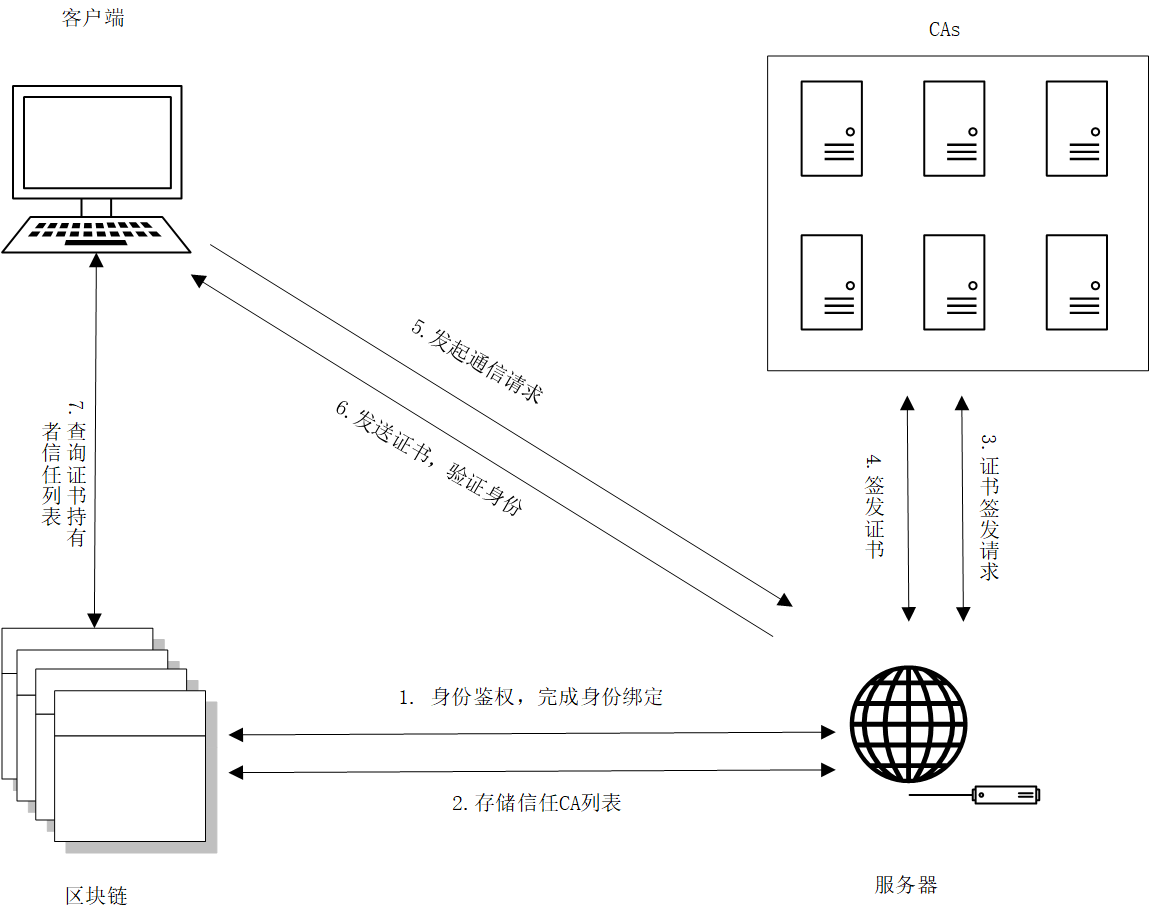
\includegraphics[width = 0.8\textwidth]{img/art}
 	\caption{总体架构}\label{fig:test}
\end{figure}


在本系统中,域名站点作为证书申请者,向区块链发起身份认证请求,当交易被记录到区块链上之后,域名站点根据请求交易提供验证信息,供验证节点对其身份进行验证;完成验证之后,域名即可将自己信任的CA列表发布到区块链上,并向自己信任的CA进行证书申请;完成申请后,即可将证书用在与用户通信的过程中,进行身份证明,此时证书验证者将通过区块链进行信任列表查询,判断该证书是否是被授权签发的。



\section{身份绑定方案}

在本方案中,域名需要将自己信任的CA列表记录到区块链上,但是区块链具有去中心化和匿名的特性,域名直接将自己的信任CA放置到区块链上是不具有可信性度,也就是说任何人都可以对任何域名进行声明。因此,之前需要完成区块链地址(或者公钥)和域名本身的绑定,实现地址与域名之间的实体认证。本文将提供基于验证时间和基于验证次数的身份绑定方案。

身份绑定过程大致分为3个步骤:

\begin{enumerate}
	\item 域名发送认证请求到区块链上;
	\item 待交易确认后,根据交易和区块在服务端放置验证;
	\item 验证节点对其进行验证,达到验证期限或者次数后,完成身份绑定。
\end{enumerate}

\subsection{基于验证时间的身份绑定方案}

基于验证时间的方案旨在让绑定者提供验证信息持续一段时间,以供所有节点对其进行验证,当提供的验证达到指定时间后,即认为其对该域名服务器的所有权,完成指定地址和域名的绑定。


\noindent\textbf{假设}

假设绑定者A拥有公钥$Pk_A$、私钥$Sk_A$以及域名$example.com$,其需要完成$(Pk_A, example.com)$的绑定;某一验证者B拥有公钥$Pk_B$和私钥$Sk_B$。

\noindent\textbf{交易类型}

在本方案中,包含以下两种类型的交易:

\begin{enumerate}
	\item 绑定请求交易$Tx_{req}$:交易请求者发布绑定请求,包含了自己的公钥$Pk_A$和域名$examle.com$。
	\item 检举交易$Tx_{rep}$:在绑定完成之前,验证节点发现绑定者的验证信息放置不准确,可以提出检举交易,驳回身份绑定。
\end{enumerate}

\noindent\textbf{流程}

绑定的具体流程包含以下四步:

\begin{enumerate}
	\item $A$发布绑定交易$Tx_{req}(Pk_A, example.com)$到区块链上;
	\item 根据需要的绑定信息$(Pk_A, example.com)$,计算$(Path, Chal) = F(Pk_A, example.com)$放置在自己控制的域名下,即访问$example.com/Path$即可获取到$Vcode = Sign_{Sk_A}(Chal)$值;
	\item 验证者$B$访问域名验证A是否正确操作,如果不,发送检举交易$Tx_{rep}(Pk_A, example.com)$到区块链;
	\item $A$保持验证时长$T$后,可停止该验证服务,完成绑定。
\end{enumerate}

在该绑定过程中,首先需要绑定者将绑定信息自己的$Pk_A$和自己的域名$example.com$发布到区块链上,将绑定身份信息展现给所有的验证节点,并根据函数$F$生成相关验证内容。我们选择哈希函数$sha256$作为函数原型,将$Pk_A$和$example.com$直接拼接后作为输入,将计算得到的256位哈希值前128位赋值给$Path$、后128位赋值给$Chal$,并且使用自己的私钥对$Chal$进行签名:

\begin{equation}\label{eqF}
Path_{128}||Chal_{128} = sha256(Pk_A||example.com)
\end{equation}

\begin{equation}\label{eqSign}
Vcode = Sign_{Sk_A}(Chal)
\end{equation}

绑定者将以上得到的$Vcode$值放置在网站的$example.com/Path$目录下,作为身份验证的内容,供所有验证节点验证。如果验证节点在验证过程中发现其并没有正确的放置验证信息,将可以通过发送检举信息$Tx_{rep}$对身份绑定消息进行驳回。


\subsection{基于验证次数的身份绑定方案}\label{ver_num}

基于验证次数的方案需要在绑定者发布绑定信息后,选择出合适的验证者,对绑定者的验证信息进行确认,当验证的次数达到规定次数后即可完成身份绑定。

\noindent\textbf{假设}

假设绑定者A拥有公钥$Pk_A$,私钥$Sk_A$以及域名$example.com$,其需要完成$(Pk_A, example.com)$的绑定;某一验证者B拥有公钥$Pk_B$和私钥$Sk_B$。

\noindent\textbf{交易类型}

在本方案由于需要特定验证者完成验证信息的确认,相比于基于时间的验证方案,增加了验证交易类型,包含一下三类交易类型:

\begin{enumerate}
	\item 绑定请求交易$Tx_{req}$:交易请求者发布绑定请求,包含了自己的公钥$Pk_A$和域名$examle.com$。
	\item 检举交易$Tx_{rep}$:在绑定完成之前,验证节点发现绑定者的验证信息放置不准确,可以提出检举交易,驳回身份绑定。
	\item 验证交易$Tx_{vfy}$:验证者在完成验证信息的对比后,在验证通过的情况下发送验证通过的交易。
\end{enumerate}

\noindent\textbf{流程}

基于验证次数的身份绑定方案相比于基于验证时间的方案需要验证者更多的和区块链进行交互,在验证过程中需要将验证是否通过的信息提交到区块链上去,具体流程如下:

\begin{enumerate}
	\item $A$发布绑定交易$Tx_{req}(Pk_A, example.com)$到区块链上;
	\item  A获取$Tx_{req}$所在位置区块信息$Info_{block}$,并根据其计算值$(Path, Chal) = F(Info_{rcvBlock})$放置在自己控制的域名下,及访问$example.com/Path$即可获取到$Vcode = Sign_{Sk_A}(Chal)$值;
	\item 根据交易$Tx_{req}$计算符合该条请求的验证者:${v_1, v_2, ... , v_k}$,假设$B$为其中一个验证者
	\item B从$example.com/Path$获取验证内容,提交交易$Tx_{vfy}(Pk_B, Pk_A, Vcode)$ 完成验证。
	\item 在经过$K$个验证过后,即完成绑定。
\end{enumerate}

整体流程和基于时间的方案类似,需要绑定者将自己的公钥$Pk_A$和自己的域名$example.com$发布到区块链上,然后通过公式函数获得\eqref{eqF}和\eqref{eqSign}计算得到$Path$和$Vcode$的值放置到自己的服务器上;验证者通过\eqref{eqF}计算获得$Path$、$Chal$和$Pk_A$对验证信息进行确认,确认通过后发送验证交易$Tx_{vry}$到区块链上完成一次验证,待达到验证次数$K$后,即完成身份绑定。

\noindent\textbf{验证者的选取}

在本方案中,需要一种选取选取验证者的规则,避免节点为了自己的利益而不纳入或者滞后其它节点的验证交易;更为重要的是,如果验证节点不是经过一定规则筛选得出的,而是每个节点都可以对绑定身份进行验证的话,在本方案中恶意的绑定者可以使用不同的公钥作为验证节点,然后对恶意绑定进行确认;同时,正常的验证者为了获得更多的奖励,也会申请尽量多的账户对交易进行验证。

为了避免以上的情况出现,本方案中设计了依据绑定信息随机选择验证节点的方法,保证验证可以有效的进行。当绑定信息被发布到区块链上后,根据绑定信息$Pk_A$、$example.com$和该交易所在位置的区块信息$Info_{rcvBlock}$,将其装换为基准值$hash_{cmp}$:

\begin{equation}\label{eqGenCmpPk}
hash_{cmp} = sha_{512}(Pk_A||example.com||Info_{rcvBlock})
\end{equation}

得到基准值之后,验证节点将通过对纳入该区块之后的区块信息进行签名,来判断自己是否具有成为验证本次交易的权力,判断的方法如\ref{cmpCondition}式所示:


\begin{equation}\label{cmpCondition}
dist_{ham}(Sha_{512}(Sig_{Pr_c}(Info_{curBlock})), hash_{cmp}) <= d + \Delta_t / t_{adjust}
\end{equation}

其中$dist_{ham}(a,b)$表示两个数a和b之间的海明距离,$d$表示初始时的海明距离要求,$\Delta_t$表示从开始收到验证请求已经过去的时间;$t_{adjust}$调整目标难度的时间;$Info_{curBlock}$表示最新块的相关信息。

以上判断方法使得一个验证者可以在每产生一个区块就可以进行一次尝试,判断自己是否能够成为验证节点,同时,随着时间的推移,成为验证节点的难度也在不断减小,保证一定会有验证者被选出。



\subsection{检举的工作机制}

在一个p2p的网络中或者一个区块链的网络中,每个用户使用都是一个公钥(即地址),和自身的身份是没有任何关系的,这就是为什么需要设计公钥与域名绑定方案的原因。但是在这样的网络中,任何人都可以发起对任意域名的绑定,为了排除一些错误的绑定或者假冒的绑定,需要设置检举的机制来完成这一目标。

当一个诚实的验证节点$C$发现一个虚假的绑定时,他就可以向区块链发起检举交易,其中包括自身的公钥$Pk_C$和绑定者公钥$Pk_A$和域名$examle.com$。但是对于一个恶意的验证节点,可能也会对一个真实有效的绑定发起检举交易。为了确认一条检举交易的有效性,需要区块链上验证节点对该条交易给出判断,和\ref{ver_num}中选择验证节点的方式类似,这里使用($Pk_C$,$Pk_A$,$example.com$)作为输入,得到一个基准地址,然后挑选出$n$个节点对该检举交易进行投票,判断该次检举的有效性。


\subsection{验证交易的附带信息}

验证交易在本方案中起着重要的作用,是验证节点参与到本系统中的重要途径之一。验证节点随时监控区块链上提交的身份绑定请求以及相对应的检举信息,当这两种消息公布到区块链上时,意味着需要验证节点参与到事件的确认当中,每个验证节点都会有机会成为验证该时间的节点。

对于身份绑定请求和检举信息的确认,同时都要提交自身的公钥$Pk_C$和绑定者的公钥$Pk_A$的公钥,不同的是一个需要提供验证内容$Vcode$,另外一个需要提供域名$example.com$。在此基础上,还需要验证者提供一个基于容量证明的内容,保证身份不是随意产生的,而是付出一定代价维护的。假设需要提供的容量证明内容为$prf$,其需要满足以下条件:

\begin{equation}\label{pocVerify}
Verify(Pk_C, prf) = Sha_512(Pk_A||Vcode/example.com||Info_{block})
\end{equation}

其中$Verify$是容量证明的验证函数。



\subsection{奖励惩罚机制}

为了促使本方案有足够多的验证节点加入,保证身份绑定能够完整有效的进行,需要对验证节点给予一定的奖励。在验证过程中,如果发现存在未合理放置验证信息的 域名,将可以发起检举交易到区块链上,待交易确认后,其可以得到相应的奖励;为保证本系统中的奖励平衡,发起绑定者需要付出一定的代价,而验证者发现错误时,将 可以获取得到相应的奖励。所以涉及到的奖励和惩罚机制包括以下几点:

\begin{itemize}
	\item 在发起绑定交易时,绑定者需要付出一定的代价
	\item 在完成验证之后,验证者将会获得相应的奖励(无论是基于验证次数方案中的验证节点或是对检举交易验证的节点)
	\item 在发起检举交易时,需要对该交易的发起付出一定担保,在检举交易确认后将退回担保
	\item 在检举交易被认可后,检举发起者和相应的验证者将会获得奖励;在检举交易被否决时,相应的验证者可以获得检举交易的担保费用
\end{itemize}

第一条规则的设计让身份绑定者需要付出代价,而不是无限制的随意的在本方案中发起身份绑定操作,从而避免了恶意的破坏者无限度的去发起无效的身份绑定,从而影响本系统中正常身份绑定者的顺利进行;第二条规则是对付出验证操作的节点给予奖励,作为吸引更多节点加入的激励机制;第三条规则是为了防止网络中的验证节点随意的发起检举交易来扰乱正常绑定的进行;第四条规则和第二条规则类似,属于激励规则,初始更多的节点加入到本系统中。同时,由于验证者在完成验证或者发现验证不通过的时候,将会获得奖励,而这些奖励不是凭空产生的,而是验证发起者所付出的相应费用。




\subsection{安全性分析}

\subsubsection{站点对域名服务器的控制权}

为了保证绑定者对域名服务器拥有控制权,在以上方案中,使用提交的$Tx_{req}$来生成验证内容$Path$和$Chal$,保证了验证内容和提交请求的相关性;同时在\eqref{eqF}中使用$sha256$作为随机函数,将提交内容转换为验证内容,该过程是一个不可逆的过程,从验证内容到提交内容的生成是很难完成的,保证了很难通过验证内容去构造提交内容。在放置的验证内容中,$Vcode$是使用绑定公钥对应私钥对$Chal$进行签名得到的,保证了绑定者对私钥的拥有权。


\subsubsection{验证交易的有效性}

基于时间的验证方案中不需要提交者发起验证提交,在发现错误的时候需要发送检举交易;对于基于验证次数的方案而言,需要提交验证内容即$Vcode$,因为有签名的存在,验证节点不能凭空的发送验证交易,需要通过服务器提供的验证信息才能正确的完成验证。

绑定者如果未能正确的放置验证内容,或者通过其它方式公布验证内容,导致验证过程依旧执行,那么其他验证节点可以通过检举交易对其发起检举。


\subsubsection{女巫攻击}

本方案建立在一个P2P的开放式网络中,任何人都可以生成公钥加入到本系统中,成为一个合法验证节点。在第二章中我们知道,一个公开且没有身份管控的开放网络很容易收到女巫攻击;更具体一点,恶意的攻击者可以生成任意多的公私钥对,从而拥有本系统的多个身份,然后在验证过程中增大自己被选为验证节点的可能性;或者恶意攻击者通过在发起绑定前,不断尝试生成公私钥对并挑选出可以成为验证节点的公私钥,然后在发起绑定交易后瞬间完成对绑定请求的确认。

对于上述的第一种情况,在本方案中的任何节点都可以生成任意多的身份,以增大自己的作为验证节点的几率。根据验证者选取公式\ref{eqGenCmpPk}可知,不仅依赖于交易的绑定信息,而且还和交易被确认在区块链上的位置密切相关,所以一个公私钥是否能成为验证者并不能事先决定。对于第二种攻击方式是一样的道理,攻击者无法事先确认成为验证者的要求。

同时,如果有人希望通过拥有多个公私钥对来发起女巫攻击,在发起验证交易还需要提供一个附加信息,其中包含了一个可验证的工作量证明。这意味着如果一个节点想拥有多个身份,就需要投入更多的空间来提供工作量证明所需的内容,很大程度上限制了一个节点所拥能拥有的身份数量。                          

\subsubsection{防定点攻击}

在本方案中,一个公私钥拥有者是否可以成为一个请求的验证者,是通过式\ref{eqGenCmpPk}和式\ref{cmpCondition}来决定。当一个请求发起之后,大家都可以得到共同的基准值$hash_{cmp}$,其无法决定一个公钥拥有者$Pk$与该基准值之间的关系,自有拥有$Pk$对应私钥$Pr$的节点才可以去计算式\ref{cmpConditon},判断自己是否能够为这一次请求进行确认操作。这意味着对于每次请求发出之后,网络中没有人能够去判断谁能为此次请求进行确认;否者,攻击者可以通过对这些确认的验证节点发起比如DDoS攻击或者劫持服务来阻止它们完成验证,进而增大自己成为验证节点的几率。

\subsubsection{验证时间的选择}

在区块链上有确认交易的概念,以保证交易被正确的收录到了区块链中,并在很大程度上达到不可篡改的安全级别\supercite{nakamoto2008bitcoin}。假设区块链上的交易确认块数为$\Delta$,出块的平均时间为$T_{avg}$,在一个$\Delta*T_{avg}$的时间之后,交易将被确认有效,在此期间,所有的节点都可以对该条交易的验证内容进行确认,一旦发现不符合的现象,即可发起检举交易,完成检举。

% \subsubsection{验证次数的选择}

% ...






\section{模块实现}

本文以以太坊为例作为区块链底层架构,利用其智能合约完成以上方案的逻辑实现,PKI各个实体通过与智能合约之间交互,存储并获取相关数据,完成对信任CA列表的读写,并最终完成对证书有效性的进一步确认。

根据上面的设计,以以太坊作为区块链基础,本系统如\ref{fig:module}图分为四个模块进行实现:智能合约、域名客户端、验证节点客户端、游览器验证插件。

\begin{figure}[htbp]
 	\centering
 	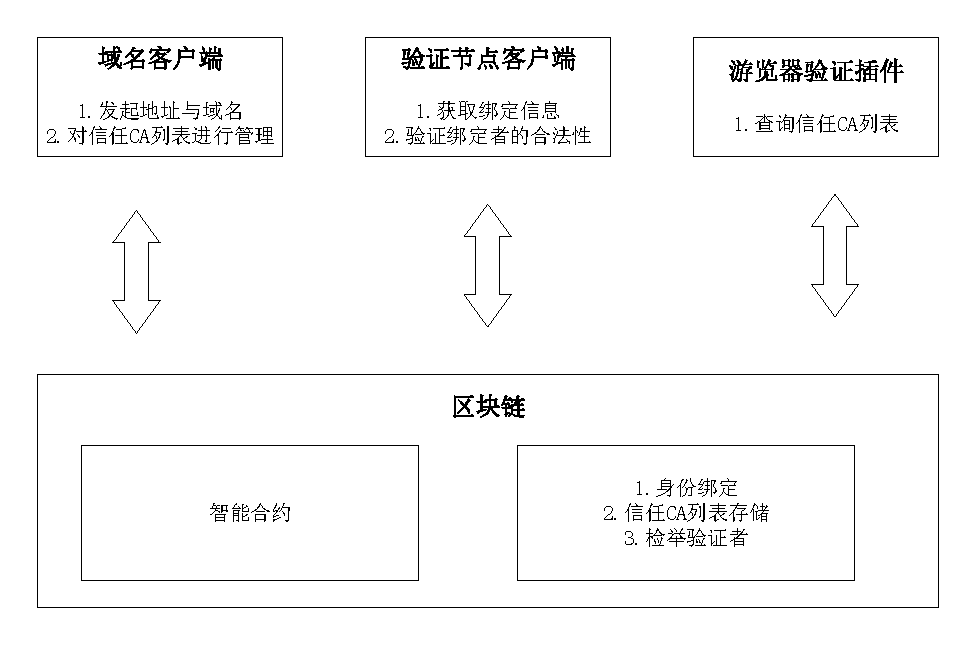
\includegraphics[width = 0.8\textwidth]{img/module}
 	\caption{系统模块}\label{fig:module}
\end{figure}

\subsection{智能合约}

智能合约作为可以在区块链上实现其他逻辑操作的一种工具,在本部分,将给予以太坊作为底层区块链基础,在其上开发具有本文所述方案的智能合约,提供其它模块访问区块链的相关接口和功能,完成本文所述方案中的逻辑操作。

在智能合约中需要提供身份绑定接口、信任列表修改接口、信任列表存储接口以及检举接口。

\subsubsection{身份绑定接口}

身份绑定接口主要提供给域名客户端和验证节点客户端使用,针对不同的客户端有两种不同的的操作:身份绑定请求和身份绑定确认。

身份绑定请求操作是由域名通过域名客户端发起,发送需要绑定的域名和公钥到智能合约中进行登记,并放置合法的验证内容到自己的服务器上,供验证节点对其进行验证。

在身份绑定请求发送成功之后,验证节点客户端可以获得最新的待验证身份绑定信息,并对身份绑定的信息进行验证,如果验证通过,则会通过智能合约调用身份绑定确认操作,完成身份绑定验证。

\subsubsection{信任列表修改接口}

域名在完成身份绑定之后,即拥有了与域名相关联的公私钥对,通过对公钥对应内容的控制调整自己信任的CA列表。其通过调用信任CA列表对信任CA进行修改操作,并存储在区块链上供其它人查阅。


\subsubsection{检举接口}

当验证者发现带确认的域名并未正确放置验证内容时,即可调用检举接口,完成对公钥对本次域名绑定的检举。

\subsection{域名客户端}

域名作为证书的申请者,需要将自己的可信任CA列表存储到区块链上,以供证书受用者在使用证书的过程中对证书的真伪进行进一步检查。

域名客户端需要与区块链进行交互,实现域名和公钥的绑定以及对自己可信CA列表的控制,主要包括以下操作:

\begin{itemize}
	\item 

	发起身份绑定请求

	通过调用智能合约身份绑定接口,发送需要绑定的域名和公钥,完成身份绑定请求操作。

	\item 

	修改信任CA列表

	在完成身份绑定之后,域名客户端将可以控制公钥和域名所对应的信任CA列表,通过调用智能合约中的信任列表修改接口,完成对自身信任CA列表的管控。


\end{itemize}

\subsection{验证节点客户端}

验证节点是本系统中身份鉴权的重要组成部分,是身份绑定有效性的保证,只有住够多验证节点存在的情况下,才可以保证身份确认的有效。

验证节点的主要工作是实时的查询验证请求并对验证请求进行验证,并根据其验证请求计算自己是否符合验证节点的要求,如果符合的话将进行验证确认操作,如果不是,也可以进行验证,对不符的验证提交检举交易。


\subsection{游览器验证插件}


游览器Web PKI中证书受用者的客户端,在原有体系结构中充当着检查证书真伪的角色。在本方案中,为了保证被恶意CA私自签发的证书可以被识别出来,需要在客户端进行对证书进行额外的检查,也就是需要游览器需要有区块链进行交互,查询收到的证书是否由证书申请者信任的CA所签发。


% vim:ts=4:sw=4
